% 黒魔術
\expandafter\ifx\csname ifdraft\endcsname\relax
    \documentclass[a4paper,twoside,12pt,papersize, dvipdfmx]{iirthesis}
    \usepackage{amsmath,amssymb,amsthm}
    \usepackage{graphicx}
    \usepackage{subcaption}
    \usepackage{url}
%    \usepackage{otf}
    \usepackage{minitoc}
    \usepackage{bm}
    \usepackage{amsmath,amssymb}
    \begin{document}

    \newcommand{\figref}[1]{\figurename\ref{#1}}
    \newcommand{\tabref}[1]{\tablename\ref{#1}}
    \renewcommand{\eqref}[1]{式~(\ref{#1})}
    \newcommand{\chapref}[1]{\ref{#1}章}
    \newcommand{\secref}[1]{\ref{#1}節}
    \newcommand{\ssecref}[1]{\ref{#1}項}
    \newcommand{\appref}[1]{付録\ref{#1}}
\fi


\chapter{平面内センサレスin-handケージングマニピュレーション}\label{chap::sicm}
\minitoc

\section{概要}
\cite{asamura2013}で,「センサレスin-handケージングマニピュレーション」という新たなマニピュレーション手法が提案された.これは,ロボットハンドの位置制御のみで対象物を拘束できる「ケージング」\cite{rimon1999}を基にしたマニピュレーション手法である.ケージングは,ロボットハンドと対象物の間の力のつり合いによって対象物を拘束する把持とは異なり,対象物の形状情報を基に幾何学的に囲い込むことで拘束する.そのため,力情報を必要としない.また,「囲い」による拘束であるため,対象物の詳細な位置情報も必要としない.一般的なIn-handマニピュレーション手法では,対象物の位置情報や力情報を必要とするが,本手法ではケージングを利用することにより,センサレスなマニピュレーションが可能となっている.\par
本手法の特徴として,上述のセンサを必要としないことに加えて,外乱に強いといった点も挙げられる.センサレスin-handケージングマニピュレーションでは,マニピュレーション中は常に対象物のケージングが成立している.そのため,マニピュレーション中に対象物に外乱が加わり位置・姿勢に変化が生じても,最後までマニピュレーションを行うことができる.\par
本手法は,センサを用いていないため,動作計画において対象物の正確な位置・姿勢情報を扱うことはできない.しかし,対象物の形状情報は既知なので,ケージングが成立している任意のハンド姿勢による囲い内において,対象物が存在できる位置・姿勢群を算出できる.そこで,ケージングに関する条件を満たしながら,囲いの形状を変化させていく過程で,対象物が存在できる位置・姿勢群の数を十分に減らし,かつ目標位置・姿勢付近へと十分に近づけることで,センサレスに対象物を目標位置・姿勢へと位置決めすることができる.\par
以下の節では,より具体的な説明を行っていく.\secref{sec::sicm::partsfeeder}では,センサレスin-handケージングマニピュレーションを行うためのシステムの説明を行う.また,新たなハンド構成の提案についても記述する.\secref{sec::sicm::cspace}では,対象物の位置・姿勢群の扱い方について,\secref{sec::sicm::caging}では,センサレスin-handケージングマニピュレーションを可能とするためのケージングに関する条件について,\secref{sec::sicm::planning}では,動作計画に使用しているアルゴリズムについて述べる.
%ケージングを用いることでセンサを必要としないこと
%オフラインで事前生成要素も書ければ書きたい

\section{汎用パーツフィーダ}\label{sec::sicm::partsfeeder}
センサレスin-handケージングマニピュレーションの位置・姿勢にばらつきのある対象物を特定の位置・姿勢に整列できるという機能を活かして,本手法はパーツフィーダへ応用することを見込んでいる.本研究では,ベルトコンベアと1対のロボットハンドを用いて\figref{fig::sicm::overview}のように構成している.ロボットハンドは,3つのリンク,3つの関節からなる3自由度ハンドとなっている.ここで,\figref{fig::sicm::overview}のように1対のロボットハンドを並列に並べたハンド構成を並列型ハンドと呼ぶこととする.
\subsection{一連の動作の流れ\cite{kamikukita2022}}\label{subsec::sicm::flow}
パーツフィーダの動作の流れについて説明する(\figref{fig::sicm::overview}).まず,ハンドを開いた状態で,ベルトコンベアにより対象物を一定時間移動させ,停止する.その後,ハンドを閉じて物体を囲み,対象物のケージング状態を作った後にマニピュレーションを行う.整列が終了すると,ハンドを開いて物体を解放し,ベルトコンベアを一定時間動かして,対象物を流出させる.\par
%本来のパーツフィーダでは,物体の分離と整列が必要となるが,本研究で扱うパーツフィーダは,物体の分離は行わず,ベルトコンベア上に十分な間隔で物体があることを前提として物体の整列動作を行う.

\begin{figure}[b]
\centering
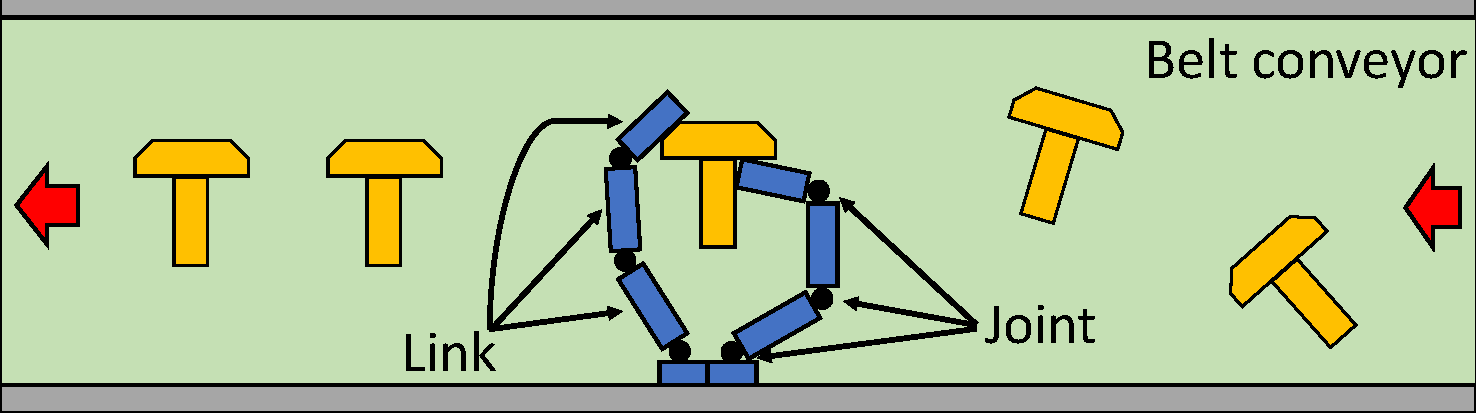
\includegraphics[width=0.9\hsize]{fig/2-sensorless-icm/systemoverview.pdf}
\caption{System overview} \label{fig::sicm::overview}
\end{figure}

\subsection{対向型ハンド}\label{subsec::sicm::oppositehand}
\secref{sec::intro::objective}で述べた通り,並列型ハンドでは対象物がハンド根元付近に詰まり,ハンドが正常に動けなくなるジャミング(\figref{fig::sicm::jam})が発生していた.また,並列型ハンドの構造上,ハンド根元関節付近に対象物が存在する場合,マニピュレーションできないといった問題点も存在した.\par
そこで,\figref{fig::sicm::opposite-hand}のようなハンド構成,対向型ハンドを提案する.
前者の問題に関して考える.並列型ハンドでは,根元付近に対象物がある場合,根元リンクのみで対象物を扱わなければならない.根元リンクは自由度が低く,発揮できる力の方向も限られている.そのため,一度ジャミングが起こると基本的にはハンドを開く方向に動かすことでしか回避できないが,通常,ハンドは目標位置・姿勢に向けて狭まっていく.これがジャミング回避が困難な理由である.一方,対向型ハンドでは手先のリンクが使える.手先リンクは自由度が高く,様々な方向へ力を発揮できる.そのため,ジャミングが起こりそうになると,それを回避するような状態が取られる.以上より,ジャミング解消が期待できる.
後者の問題に関して,対向型ハンドでは,縦方向にはどの場所に対象物が存在してもマニピュレーションすることができる.しかし,横方向は並列型ハンドほど広く扱えない.しかし,横方向の移動はベルトコンベアで賄えるので,大きな問題ではないと考えている.
\begin{figure}[b]
	\centering
	\begin{minipage}{0.33\hsize}
	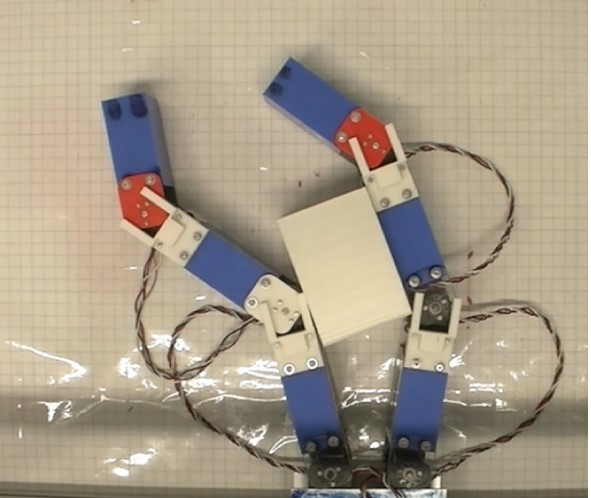
\includegraphics[width=0.9\hsize]{fig/2-sensorless-icm/jam1.jpg}
	\subcaption{Before jam}\label{fig::sicm::beforejam}
	\end{minipage}\hfill
	\begin{minipage}{0.33\hsize}
	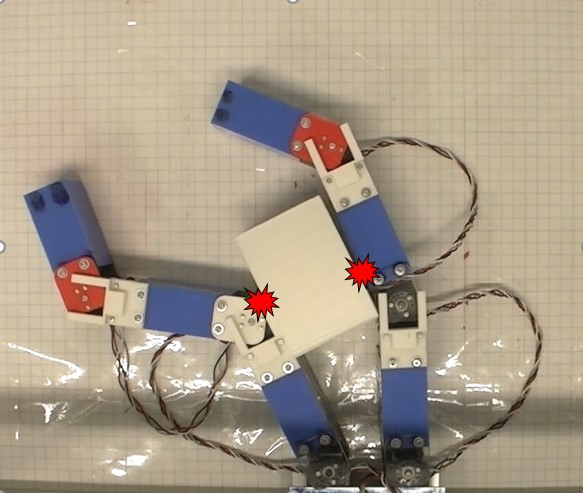
\includegraphics[width=0.9\hsize]{fig/2-sensorless-icm/jam2.jpg}
	\subcaption{Just jammed}\label{fig::sicm::justjam}
	\end{minipage}\hfill
	\begin{minipage}{0.33\hsize}
	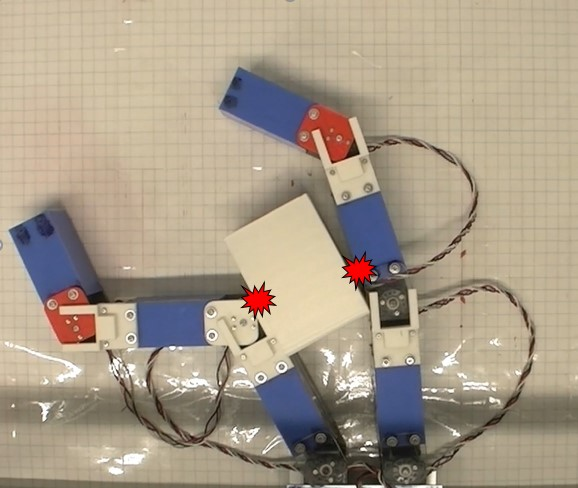
\includegraphics[width=0.9\hsize]{fig/2-sensorless-icm/jam3.jpg}
	\subcaption{Still jammed}\label{fig::sicm::stilljam}
	\end{minipage}
	\caption{Manipulation by parallel-type hand (Jamming occuring)}
	\label{fig::sicm::jam}
	

	\centering
	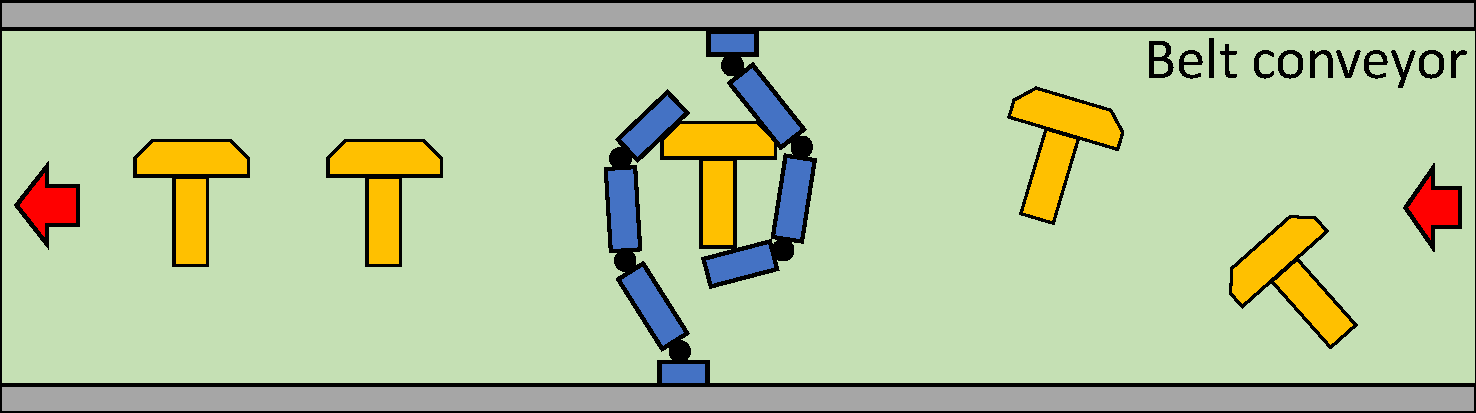
\includegraphics[width=0.9\hsize]{fig/2-sensorless-icm/opposite-type.pdf}
	\caption{Opposite-type hand} \label{fig::sicm::opposite-hand}
\end{figure}

\section{対象物のコンフィギュレーション空間\cite{komiyama2021}}\label{sec::sicm::cspace}
本節では,ハンド動作計画の際に使用する,対象物のコンフィギュレーション空間について説明する.我々は対象物の状態を,位置$(x, y)$と姿勢(傾き)$\phi$の3変数によって表している.この3変数で構成される3次元空間が対象物のコンフィギュレーション空間である.空間内の任意の座標は,対象物の任意の位置・姿勢を表しており,それぞれ1:1に対応している.\par

このコンフィギュレーション空間の中から,対象物が存在できる領域を対象物のコンフィギュレーション自由空間と呼び,$C_{\mathrm{free}}$と表す.具体的な$C_{\mathrm{free}}$の導出は以下の通りである.まず,任意の座標$(x, y, \phi)$に対して,対象物の代表点を$(x, y)$に合わせ,$\phi$だけ傾ける.このとき\figref{fig::sicm::cfree}(a)のようにハンドにも壁にも干渉しない場合,任意の座標$(x, y, \phi)$は$C_{\mathrm{free}}$を構成する点として認められ,\figref{fig::sicm::cfree}(b)のように干渉した場合は,$C_{\mathrm{free}}$を構成する点としては認めない.この判定を空間全体に対して行ったときの前者の集合が$C_{\mathrm{free}}$となる.
\begin{figure}[b]
\begin{minipage}{0.5\hsize}
\centering
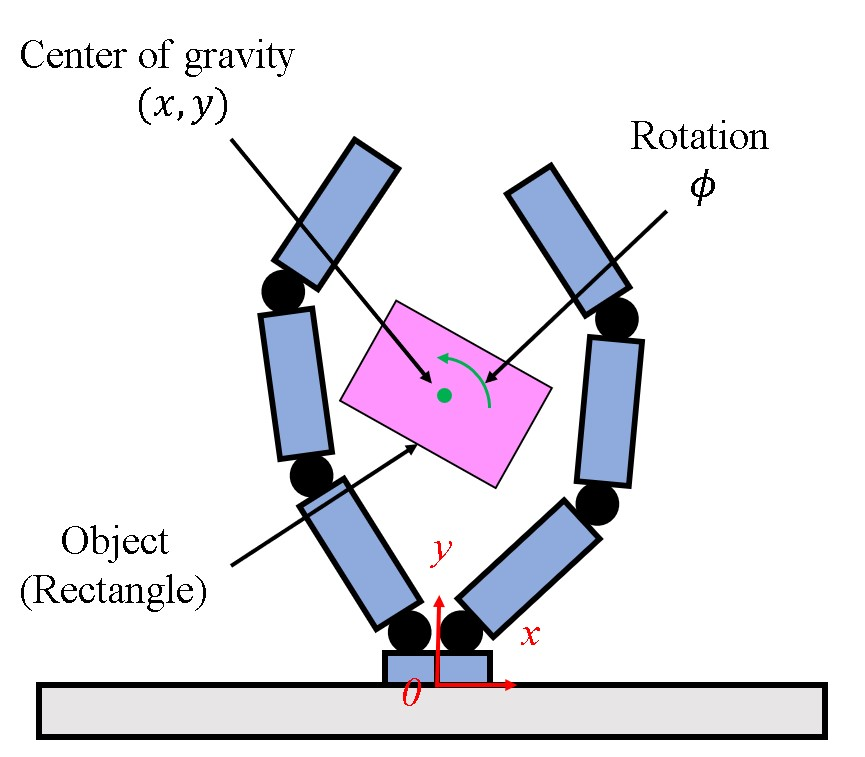
\includegraphics[width=0.9\hsize]{fig/2-sensorless-icm/define_cfree.jpg}
\end{minipage}
\begin{minipage}{0.5\hsize}
\centering
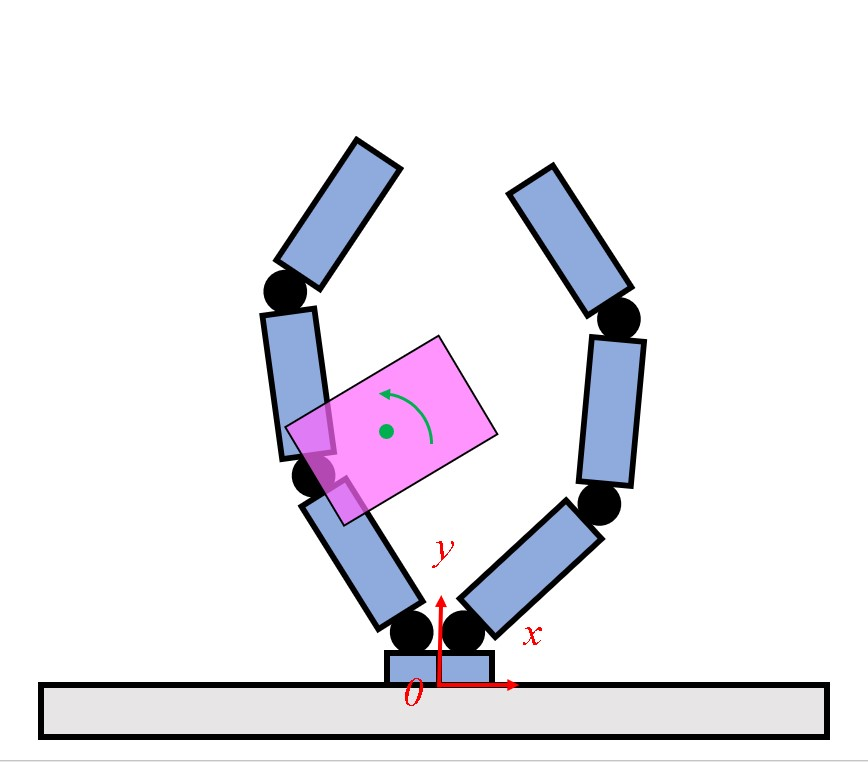
\includegraphics[width=0.9\hsize]{fig/2-sensorless-icm/define_notcfree.jpg}
\end{minipage}
\caption{Definition of $C_{\mathrm{free}}$}
\label{fig::sicm::cfree}
\end{figure}

実装にあたり,対象物のコンフィギュレーション空間を\figref{fig::sicm::discretize}のように格子状に分割し,離散的に取り扱っている.本来,コンフィギュレーション空間は連続した空間である.そのため,格子点の幅を狭めれば狭めるほど実際の表現に近くなる.一方で,格子点幅を狭めすぎると格子点数が増え,その分計算負荷が大きくなる.したがって,マニピュレーションの動作計画に支障のない範囲で格子点幅を確保しつつ,計算負荷も抑えられるようなバランスの良いパラメータ設定が重要となる.\par

一例として,6自由度並列型ハンドで長方形物体をケージングした際の対象物コンフィギュレーション$C_{\mathrm{free}}$を\figref{fig::sicm::cfreeexam}に示す.緑色領域が$C_{\mathrm{free}}$であり,この$C_{\mathrm{free}}$を評価することで,現在のハンド姿勢がセンサレスin-handケージングマニピュレーションするにあたって,妥当な姿勢か否かを判定する.この判定については,次節で説明する.

\begin{figure}[hb]
\centering
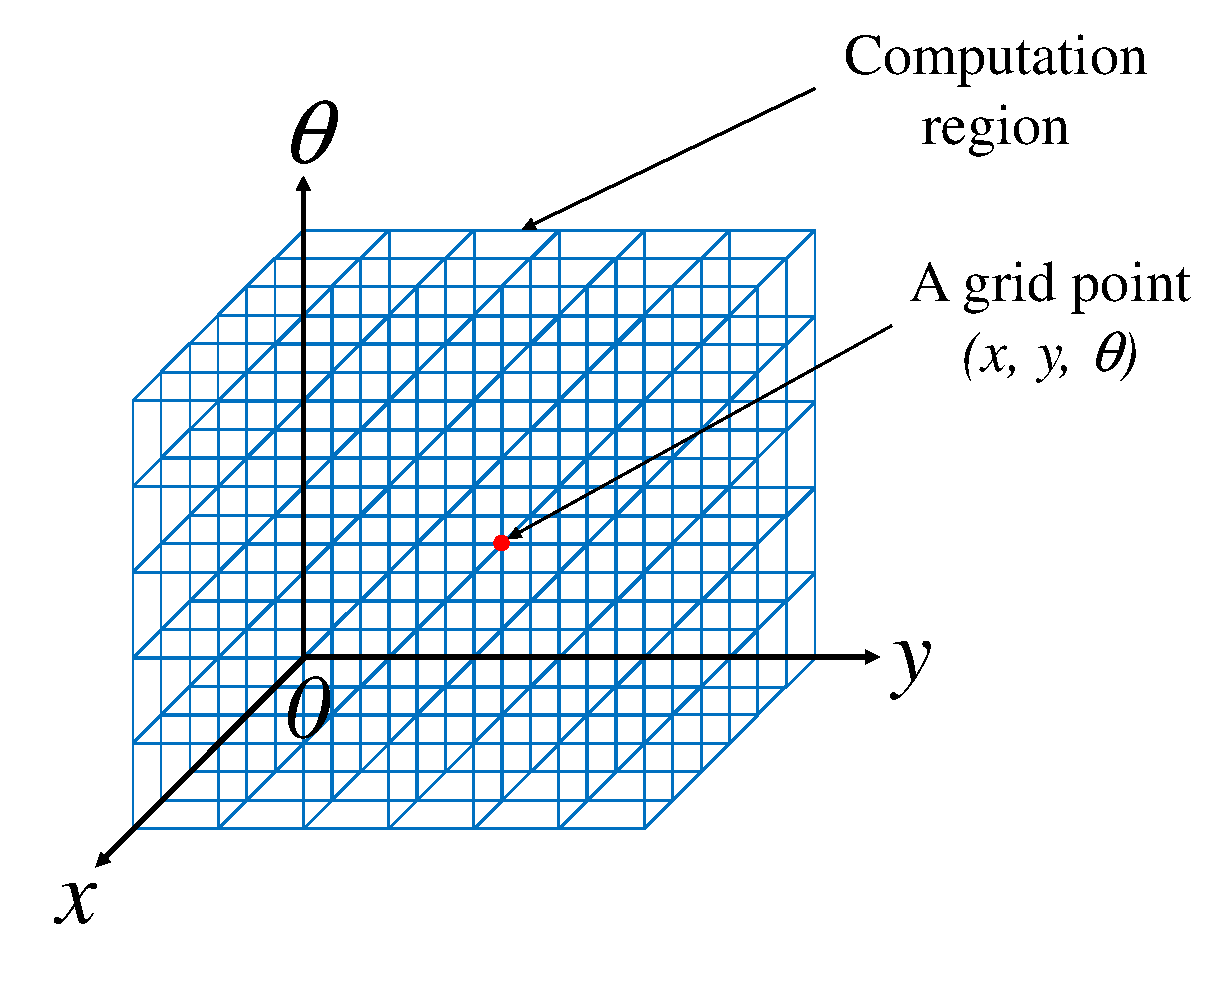
\includegraphics[width=0.6\hsize]{fig/2-sensorless-icm/DiscretizeSpace.pdf}
\caption{Discretization of the 3D computation region \cite{komiyama2021}}
\label{fig::sicm::discretize}

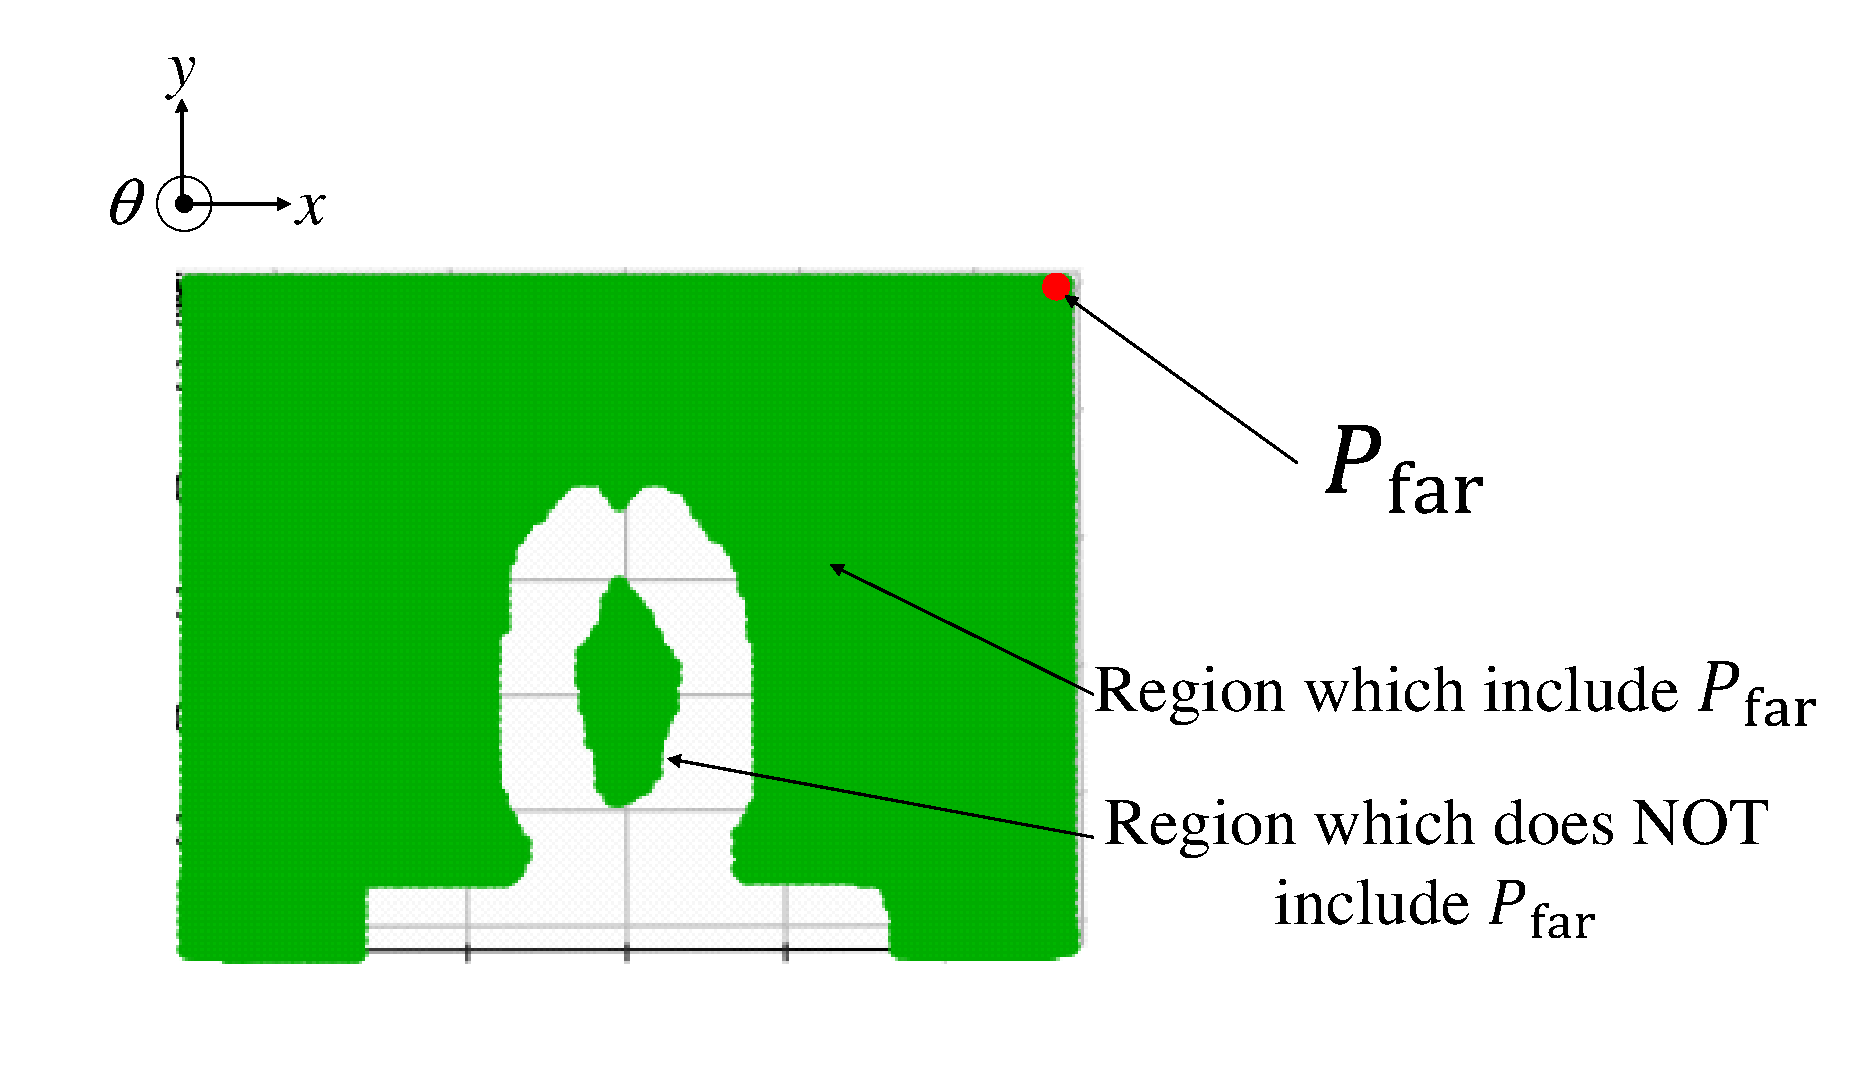
\includegraphics[width=0.7\hsize]{fig/2-sensorless-icm/cfree.pdf}
\caption{The configuration free space ($\mathcal{C}_{\mathrm{free}}$) of the object \cite{komiyama2021}}
\label{fig::sicm::cfreeexam}
\end{figure}


\section{ケージング成立条件とケージングマニピュレーション可能条件\cite{komiyama2021}}\label{sec::sicm::caging}
\subsection*{ケージング成立条件}
ケージング条件の説明にあたり,以下のように記号を定義する.
\begin{itemize}
\item $\mathcal{C}$: 物体のコンフィギュレーション空間
\item $\mathcal{A}_{\mathrm{obj}}$: 実空間での物体の領域
\item $\mathcal{A}_{\mathrm{finger}}$: 実空間でのロボットハンドの指部分の領域
\item $\mathcal{A}_{\mathrm{palm}}$: 実空間でのロボットハンドのパームの領域
\item $\bm{q}_{\mathrm{obj}}$: 物体のコンフィギュレーション
\item $\bm{q}_{\mathrm{finger}}$: ハンドの指部分のコンフィギュレーション
% \item $\bm{q}_{\mathrm{goal}}$: ハンドの指部分の目標コンフィギュレーション
\end{itemize}

まず,\secref{sec::sicm::cspace}で述べた,対象物がハンドやロボットと干渉せず存在できる位置・姿勢群であるコンフィギュレーション自由空間$\mathcal{C}_{\mathrm{free}}$は,上記の記号を用いて次のように表される.
\begin{gather}
\mathcal{C}_{\mathrm{free}} :=
\{\bm{q}_{\mathrm{obj}} \in \mathcal{C} | \mathcal{A}_{\mathrm{obj}}(\bm{q}_{\mathrm{obj}})
\cap \mathcal{A}_{\mathrm{finger}}(\bm{q}_{\mathrm{finger}}) \neq \varnothing\}
\label{eq::cfree}
\end{gather}

対象物のケージングが成立している場合,\figref{fig::sicm::cfreeexam}のように$\mathcal{C}_{\mathrm{free}}$は少なくとも2つ以上の連結した領域に分割される.これらの領域の集合を$\mathcal{C}_{\mathrm{free\_cluster}}$と表す.$\mathcal{C}_{\mathrm{free\_cluster}}$は2つのグループに分けられる.1つは,ハンドによって囲われ,ハンド内部で独立している領域.もう1つは,ハンド外部と接続された領域である.前者は対象物がハンド内部から出ることができないことを意味するためICS (Inescapable Configuration Space)と,後者は対象物がハンド外部へ自由に逃げられることを意味するためECS (Escapable Configuration Space)と呼ぶ(\figref{fig::sicm::cfreeics}).これらに属するコンフィギュレーション自由空間をそれぞれ$\mathcal{C}_{\mathrm{free\_ICS}}$,$\mathcal{C}_{\mathrm{free\_ECS}}$と定義する.$\mathcal{C}_{\mathrm{free\_ICS}}$,$\mathcal{C}_{\mathrm{free\_ECS}}$は,以下のような式で表される.


\begin{gather}
%\mathcal{C}_{\mathrm{free\_ECS}} := 
%\bigcup_{\bm{q}_{\mathrm{obj}}\in \mathcal{P}_{\mathrm{far}}}
%\mathcal{C}_{\mathrm{free\_max}}(\bm{q}_{\mathrm{obj}}) \\
\mathcal{C}_{\mathrm{free\_ECS}} := 
 \{\mathcal{C}_{\mathrm{free\_cluster}} \ni \mathcal{C}_{\mathrm {free}} | \mathcal{C}_{\mathrm{free\_cluster}} \ni \mathcal{P}_{\mathrm {far}}\} \\
\mathcal{C}_{\mathrm{free\_ICS}} := \mathcal{C}_{\mathrm{free}} 
\setminus \mathcal{C}_{\mathrm{free\_ECS}}
\end{gather}

ここで,$\mathcal{P}_{\mathrm{far}}$は,無限遠点の集合を指す.ここで,ロボットハンドによって囲われる可能性のない程度に離れた点も,無限遠点につながるという観点から無限遠点として扱う.実際には$\mathcal{C}_{\mathrm{free}}$の内,$\mathcal{P}_{\mathrm{far}} (\subset \mathcal{C})$を含む領域を$\mathcal{C}_{\mathrm{free\_ECS}}$と,$\mathcal{P}_{\mathrm{far}} (\subset \mathcal{C})$を含まない領域を$\mathcal{C}_{\mathrm{free\_ICS}}$と判定する.\par

$\mathcal{C}_{\mathrm{free\_ICS}}$は複数の領域から構成される場合がある.言い換えると,対象物がハンド内部で取りうる位置・姿勢群は数パターンある場合がある.この内,実際に対象物が存在している領域はいずれか一つであり,この領域を$\mathcal{C}_{\mathrm{free\_obj}}$と定義する.式では以下のようにあらわせる.
\begin{gather}
\mathcal{C}_{\mathrm{free\_obj}} \subseteq \mathcal{C}_{\mathrm{free\_ICS}}
\end{gather}

ここで,センサレスに$\mathcal{C}_{\mathrm{free\_obj}}$領域を特定するため,$\mathcal{C}_{\mathrm{free\_obj}}$の連続性を考える.つまり,対象物が実際に取りうる位置・姿勢群$\mathcal{C}_{\mathrm{free\_obj}}$は,直前$(t-\Delta t)$のハンド姿勢のものと現在$(t)$のハンド姿勢のものでは連続性の観点からオーバーラップしていると考える(\eqref{eq::sicm::continuous}).
\begin{gather}\label{eq::sicm::continuous}
\mathcal{C}_{\mathrm{free\_obj}}(t-\Delta t) \cap 
\mathcal{C}_{\mathrm{free\_obj}}(t) \neq \varnothing
\end{gather}
これを基に,$\mathcal{C}_{\mathrm{free\_obj}}(t-\Delta t)$とオーバーラップする$\mathcal{C}_{\mathrm{free\_ICS}}(t)$を取り出すことで,$\mathcal{C}_{\mathrm{free\_obj}}(t)$が抽出される.$\mathcal{C}_{\mathrm{free\_obj}}(t=0)$は既知であるため,全ての時刻$t$において帰納的に特定できる.

ケージング成立条件は,対象物が実際に取りうる位置・姿勢群がハンドによって完全に囲われ,外部に逃げられないことを保証するもので,以下の式で表せる.
\begin{gather}
\mathcal{C}_{\mathrm{free\_obj}} \neq \varnothing
\end{gather}

\begin{figure}[hb]
\centering
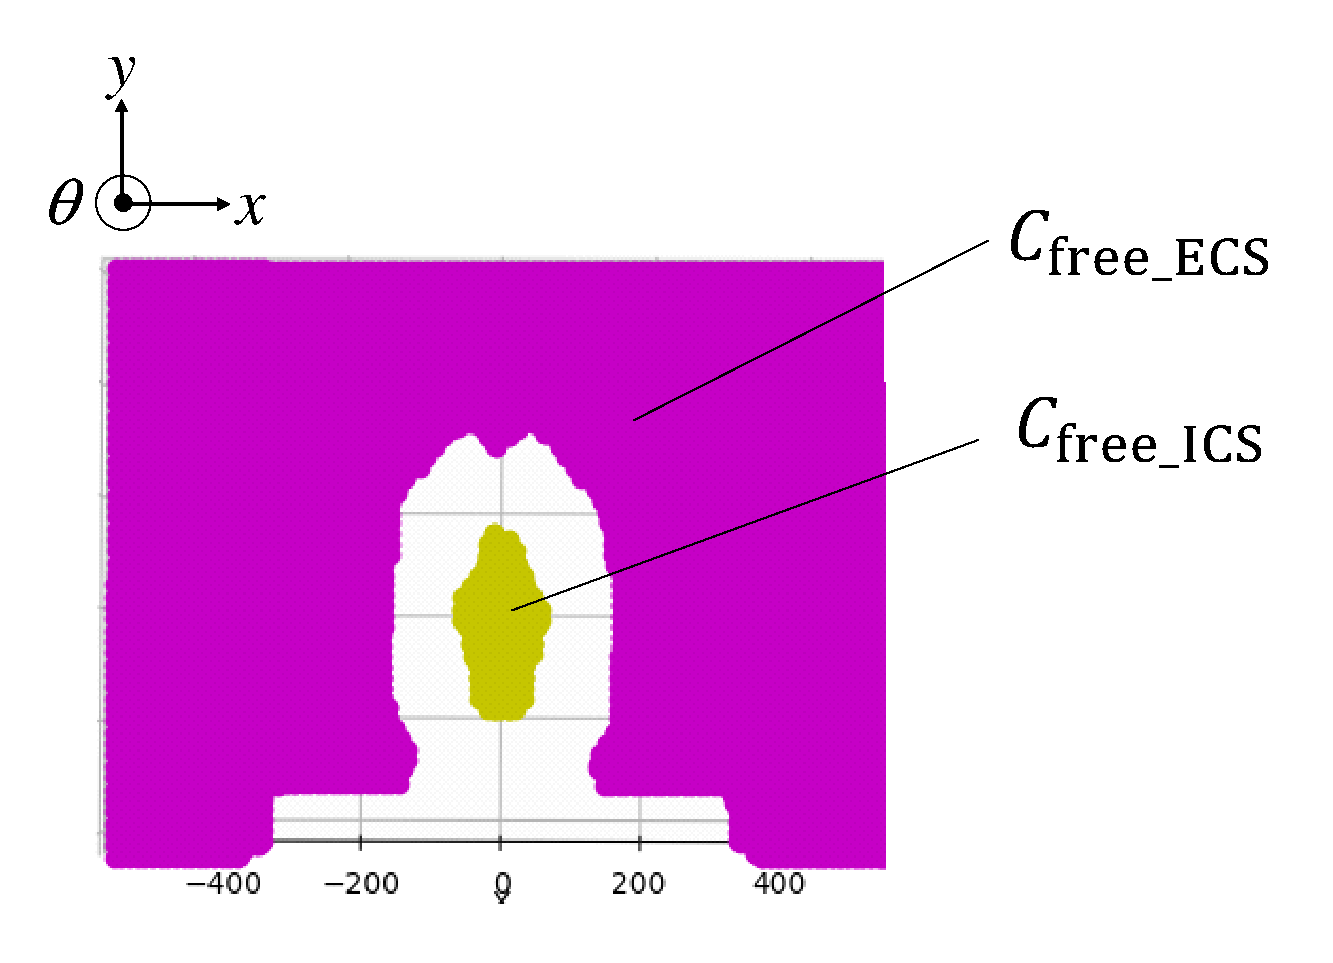
\includegraphics[width=0.6\hsize]{fig/2-sensorless-icm/cfree_ics.pdf}
\caption{$\mathcal{C}_{\mathrm{free}}$ can be classified into $\mathcal{C}_{\mathrm{free\_ICS}}$ or $\mathcal{C}_{\mathrm{free\_ECS}}$ \cite{komiyama2021}}\label{fig::sicm::cfreeics}
\end{figure}

\clearpage
\subsection*{ケージングマニピュレーション可能条件}
ケージングマニピュレーション可能条件とは,センサレスな本手法において対象物の状態を確実に追跡するための条件である.先述の方法で,$\mathcal{C}_{\mathrm{free\_obj}}(t)$の抽出を行うと,複数の領域が得られる場合がある.この場合,対象物が$\mathcal{C}_{\mathrm{free\_obj}}(t-\Delta t)$から実際にどの領域へ遷移したか特定できない.この状態が続くと,対象物を最終的な目標位置・姿勢へマニピュレーションできなくなる.このような事態を防ぐため,以下の条件をケージングマニピュレーション可能条件として定めている.
\begin{itemize}
\item $\mathcal{C}_{\mathrm{free\_obj}}$が1つの領域のみにより構成される
\end{itemize}

\figref{fig::scim::divided1},\figref{fig::sicm::divided2}は,ハンド姿勢のわずかな変化で$\mathcal{C}_{\mathrm{free\_obj}}$が二つの領域に分裂する場合の例を示している.\par
$\mathcal{C}_{\mathrm{free\_obj}}$が一度分裂しても,後のハンド姿勢の変化によって,分裂した領域が再び一つになる場合がある.このような場合,それ以後のマニピュレーションは問題なく進むものと考えられるが,動作計画の際に,分裂した$\mathcal{C}_{\mathrm{free\_obj}}$の領域全てを追跡することは,非常に多くの計算量を要する作業である.そのため,一度$\mathcal{C}_{\mathrm{free\_obj}}$が分裂した時点で,当該ハンド姿勢は妥当ではないとしてハンドの動作を計画した.

\begin{figure}[b]
    \centering        
    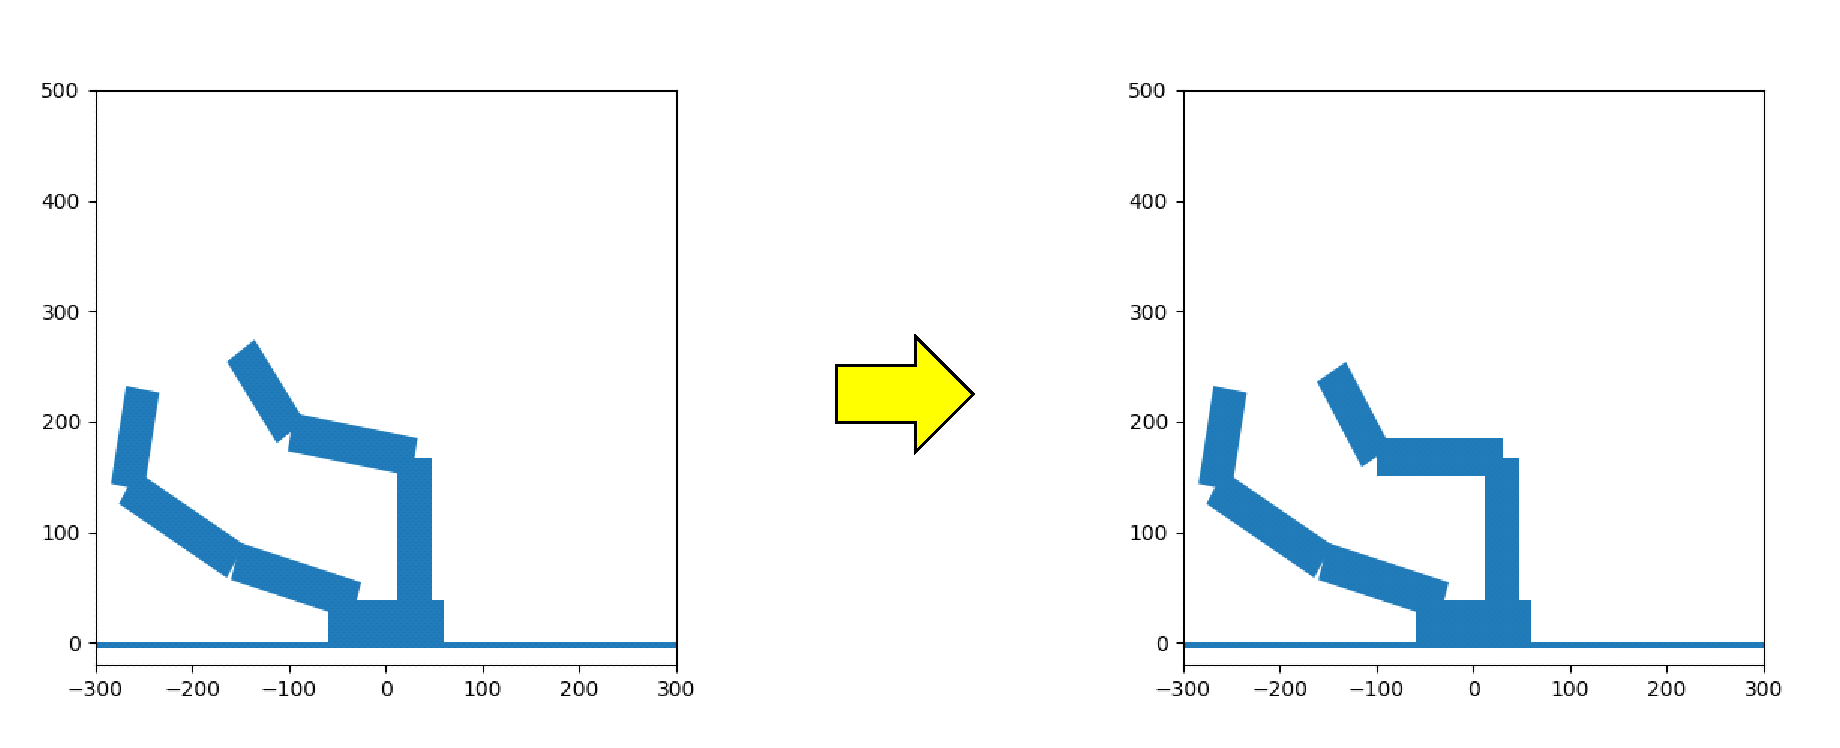
\includegraphics[width=0.8\hsize]{fig/2-sensorless-icm/cfree_obj_divided1.pdf}
    \caption{The posture of the hand when the $\mathcal{C}_{\mathrm{free\_obj}}$ is divided into multiple connected regions \cite{komiyama2021}}
    \label{fig::scim::divided1}

    \centering
    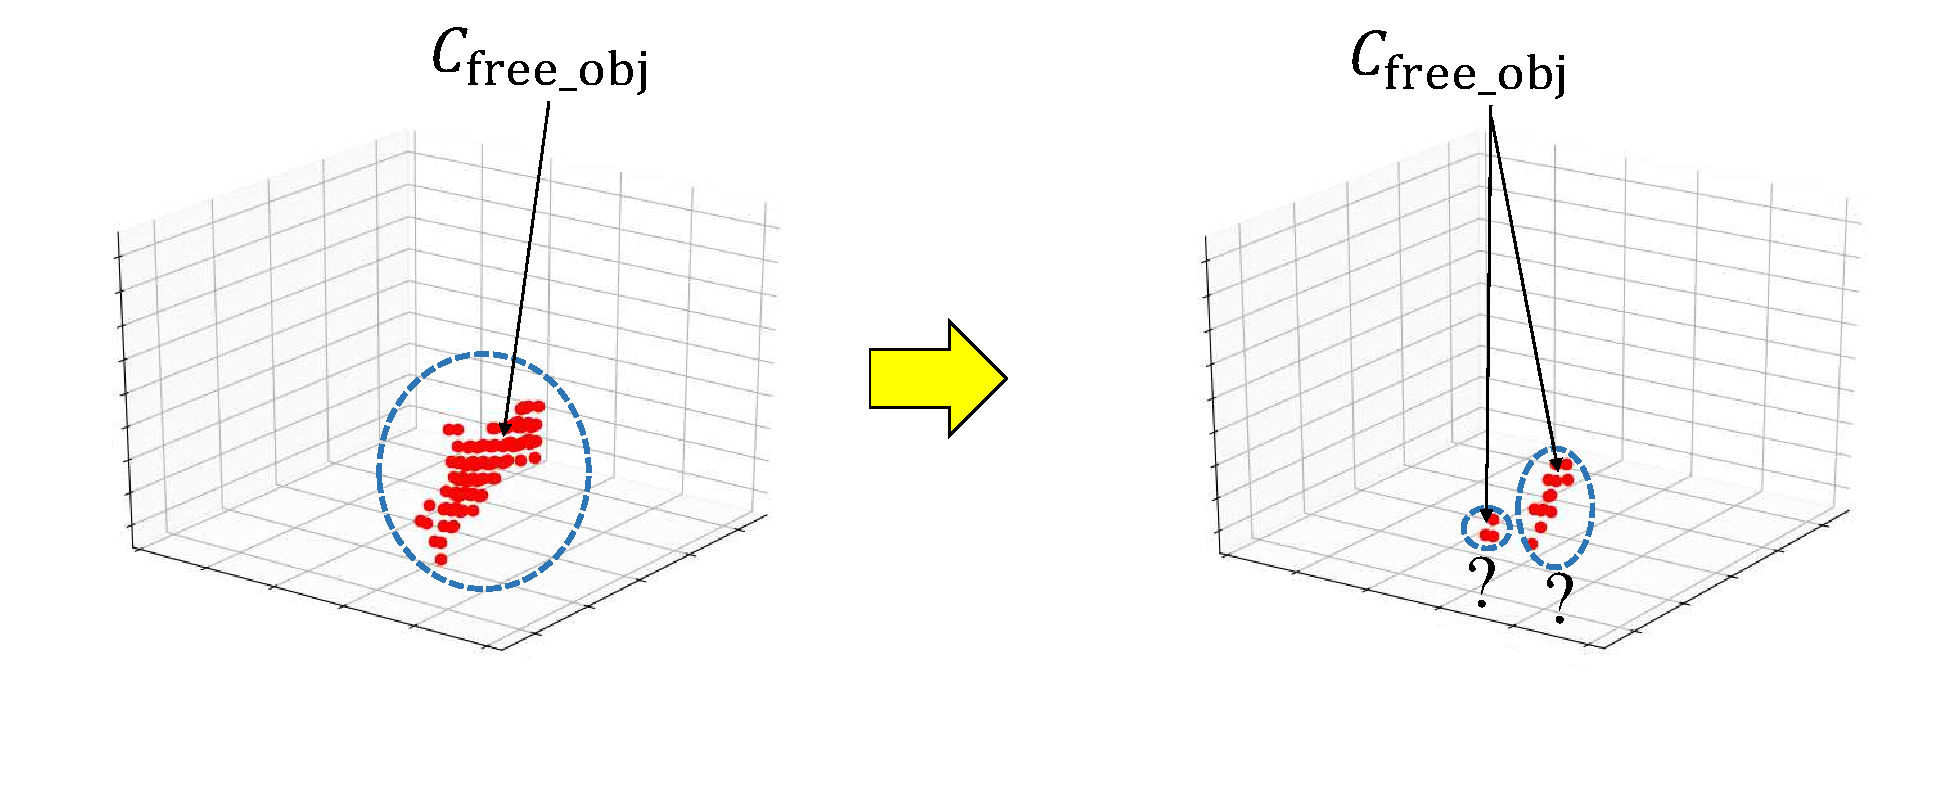
\includegraphics[width=0.85\hsize]{fig/2-sensorless-icm/cfree_obj_divided2.pdf}
    \caption{$\mathcal{C}_{\mathrm{free\_obj}}$, in the postures of the hand in \figref{fig::scim::divided1}, is divided into multiple connected regions \cite{komiyama2021}}
    \label{fig::sicm::divided2}
\end{figure}

\section{ハンドの動作計画\cite{komiyama2021}}\label{sec::sicm::planning}
先述の通り,本手法ではケージング成立条件とケージングマニピュレーション可能条件を満たした状態を維持しつつハンドを動かすことで,センサレスに対象物を目標位置・姿勢へとマニピュレーションできる.本節では,このハンドの動作生成について説明する.\cite{komiyama2021}では,経路計画手法の一つであるRRT (Rapidly-exploring Random Trees) \cite{lavalle2001}を用いた.ここで,ハンド動作はあらかじめオフラインで生成している.具体的なアルゴリズムは以下の通りである.
\begin{enumerate}
\item ハンドの初期ノード(姿勢)$\bm{q}_{\mathrm{initial}}$を設定する
\item ハンドの任意のノード$\bm{q}_{\mathrm{sample}}$をサンプリングし,$\bm{q}_{\mathrm{sample}}$から最も近いノード$\bm{q}_{\mathrm{nearest}}$を見つける\label{algo::sampling}
\item $\bm{q}_{\mathrm{nearest}}$から$\bm{q}_{\mathrm{sample}}$の方向へ長さ$\Delta l$の枝を伸ばし,そのノードを$\bm{q}_{\mathrm{new}}$とする
\item $\bm{q}_{\mathrm{new}}$において環境とハンドまたはハンド同士の干渉があれば手順\ref{algo::sampling}に戻る
\item $\bm{q}_{\mathrm{new}}$においてケージング成立条件を満たさなければ手順\ref{algo::sampling}に戻る
\item $\bm{q}_{\mathrm{new}}$においてケージングマニピュレーション可能条件を満たさなければ手順\ref{algo::sampling}に戻る
\item $\bm{q}_{\mathrm{nearest}}$から$\bm{q}_{\mathrm{new}}$へ枝を伸ばす\label{algo::fin}
\item 手順\ref{algo::sampling}から手順\ref{algo::fin}を繰り返し,$\bm{q}_{\mathrm{new}}$が終了条件を満たせば探索終了とする \label{algo::goal}
\end{enumerate}
これにより,ハンドの初期姿勢から終了姿勢までの一連の時系列データが得られる.
\begin{figure}[b]
\centering
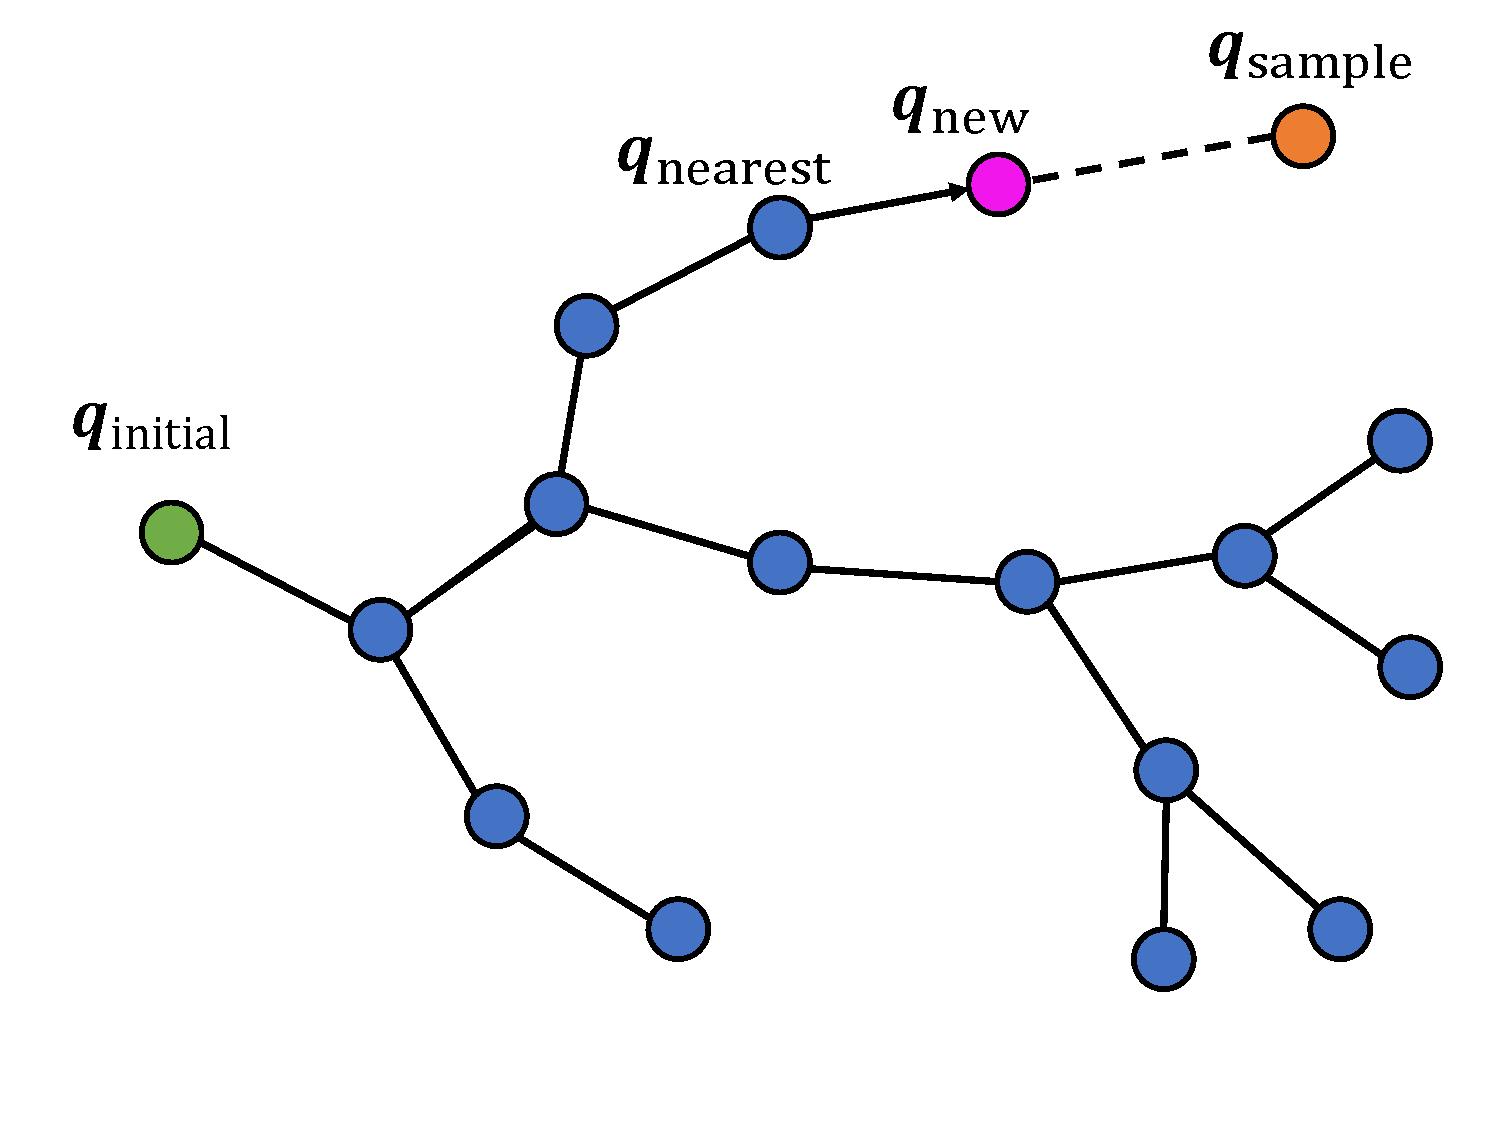
\includegraphics[width=0.5\hsize]{fig/2-sensorless-icm/rrtdiagram.pdf}
\caption{Procedure of RRT \cite{komiyama2021}}
\label{fig::sicm::rrt}
\end{figure}

手順\ref{algo::goal}の探索終了条件の説明にあたり,収束度$e$を定義する.収束度$e$は,その時のハンド姿勢によって対象物が目標位置・姿勢へどの程度,位置決めされているかを示すもので以下の\eqref{eq::sicm::e}で表される.$e$の値が小さければ小さいほど,位置決め精度が高いことを意味する.
\begin{gather}
e = \max \sqrt{(w_1(x-x_{\mathrm{goal}}))^2+(w_2(y-y_{\mathrm{goal}}))^2 + (w_3(\phi-\phi_{\mathrm{goal}}))^2}\label{eq::sicm::e} \\
(x, y, \phi) \in \mathcal{C}_{\mathrm{free\_obj}} \notag
\end{gather}
ここで,$w_1$,$w_2$,$w_3$は定数であり,これらによって\eqref{eq::sicm::e}の各項を無次元化し,位置$(x, y)$と姿勢$\phi$という異なる単位同士を一つの式で取り扱えるようにしている.\par
そして,収束度$e$と閾値$\varepsilon$を用いて探索終了条件は以下の\eqref{eq::sicm::goalcondition}となっている.
\begin{gather}
\label{eq::sicm::goalcondition}
e \leq \varepsilon 
\end{gather}
閾値$\varepsilon$を小さくする,つまり位置決め精度を高めようとすると計算時間が長くなり,閾値$\varepsilon$を大きくすると計算時間が短くなる.すなわち,位置決め精度と計算時間の間にはトレードオフの関係があり,両者のバランスを取ったパラメータ設定が重要となる.

% 白魔術
\expandafter\ifx\csname ifdraft\endcsname\relax
    \end{document}
\fi
